\documentclass[tikz,border=2pt]{standalone}
\usepackage{amsmath,amssymb}
\usepackage{pgfplots}
\pgfplotsset{compat=1.18}
\usetikzlibrary{arrows.meta}
\begin{document}
% PGF of N ~ Poisson(2): G_N(z) = e^{2(z-1)} on [0,1]; G_N(0) = P(N=0) = e^{-2}, G_N(1) = 1,
% and the tangent at z = 1 has slope G_N'(1) = E[N] = 2.
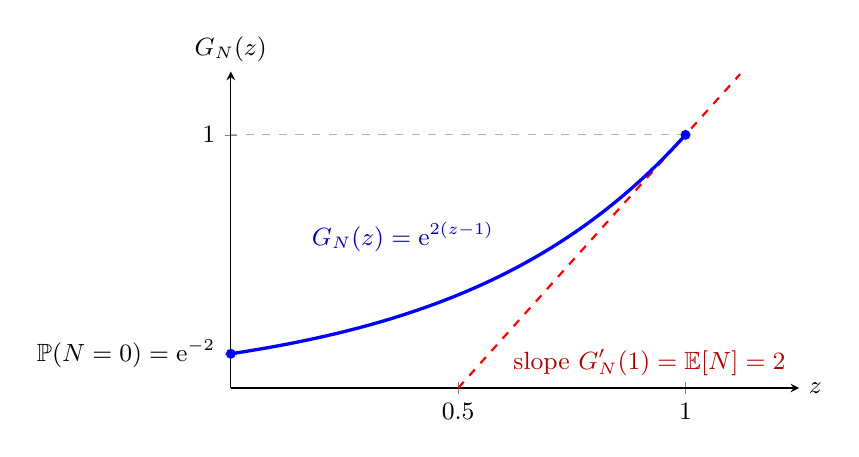
\begin{tikzpicture}[font=\small, >={Latex[length=2mm]}]
  \begin{axis}[
    axis lines=left, xmin=0, xmax=1.25, ymin=0, ymax=1.25,
    xtick={0.5,1}, ytick={0.135,1}, yticklabels={$\mathbb{P}(N=0)=\mathrm{e}^{-2}$,$1$},
    xlabel={$z$}, ylabel={$G_N(z)$},
    xlabel style={at={(axis description cs:1,0)}, anchor=west},
    ylabel style={rotate=-90, at={(axis description cs:0,1)}, anchor=south},
    samples=100, width=8.8cm, height=5.6cm, clip=false]
    \addplot[red, thick, dashed, domain=0.5:1.12] {1+2*(x-1)};
    \addplot[blue, very thick, domain=0:1] {exp(2*(x-1))};
    \draw[gray!60, thin, dashed] (axis cs:1,1) -- (axis cs:0,1);
    \fill[blue] (axis cs:0,0.1353) circle (1.8pt);
    \fill[blue] (axis cs:1,1) circle (1.8pt);
        \node[blue!70!black, anchor=south east] at (axis cs:0.6,0.5) {$G_N(z)=\mathrm{e}^{2(z-1)}$};
    \node[red!70!black, anchor=west] at (axis cs:0.6,0.1) {slope $G_N'(1)=\mathbb{E}[N]=2$};
  \end{axis}
\end{tikzpicture}
\end{document}
